% =====================================================================
%  Cerebro Cuantico Optogenetico -- Quantum walks sobre el conectoma (version breve)
%  Compilar con:  pdflatex teoria_cerebro_cuantico.tex  (dos veces)
%  Version larga (circuitos, IonQ, ruido): teoria_extendida.tex
%  Figuras en:    figuras/  (generadas con el codigo de qollab/cerebro_q)
% =====================================================================
\documentclass[11pt,a4paper]{article}

\usepackage[utf8]{inputenc}
\IfFileExists{lmodern.sty}{\usepackage{lmodern}\usepackage[T1]{fontenc}}{}
\IfFileExists{spanish.ldf}%
  {\usepackage[spanish,es-noshorthands,es-tabla,es-nodecimaldot]{babel}}%
  {\usepackage[english]{babel}% respaldo si falta el castellano: mismos nombres
   \addto\captionsenglish{\renewcommand{\figurename}{Figura}\renewcommand{\tablename}{Tabla}%
     \renewcommand{\contentsname}{Índice}\renewcommand{\abstractname}{Resumen}%
     \renewcommand{\refname}{Referencias}\renewcommand{\appendixname}{Apéndice}}}
\usepackage[margin=2.5cm]{geometry}
\usepackage{amsmath,amssymb,amsthm,mathtools}
\usepackage{bm}
\usepackage{graphicx}
\usepackage{booktabs}
\usepackage{array}
\newcolumntype{L}[1]{>{\raggedright\arraybackslash}p{#1}}
\usepackage{xcolor}
\usepackage{tikz}
\usetikzlibrary{arrows.meta,positioning,shapes.geometric,fit,calc}
\usepackage{quantikz}
\usepackage{listings}
\usepackage[most]{tcolorbox}
\usepackage[expansion=false]{microtype}
\usepackage[hidelinks]{hyperref}
\usepackage{cleveref}

% ---------------------------------------------------------------- colores
\definecolor{azul}{HTML}{2A78D6}
\definecolor{naranjo}{HTML}{EB6834}
\definecolor{verde}{HTML}{1BAF7A}
\definecolor{violeta}{HTML}{6250D6}
\definecolor{tinta}{HTML}{52514E}

% ---------------------------------------------------------------- notación
% quantikz ya define \ket y \bra; se redefinen con la misma notación
\renewcommand{\ket}[1]{\lvert #1\rangle}
\renewcommand{\bra}[1]{\langle #1\rvert}
\newcommand{\bk}[2]{\langle #1\vert #2\rangle}
\renewcommand{\proj}[1]{\lvert #1\rangle\!\langle #1\rvert}
\newcommand{\vac}{\ket{\mathbf{0}}}
\newcommand{\e}{\mathrm{e}}
\newcommand{\ii}{\mathrm{i}}
\newcommand{\tr}{\operatorname{Tr}}
\newcommand{\hop}{\mathrm{hop}}
\newcommand{\TVD}{\mathrm{TVD}}
\newcommand{\Nop}{\hat N}
\newcommand{\RX}{R_X}
\newcommand{\RXX}{R_{XX}}
\newcommand{\RYY}{R_{YY}}
\newcommand{\code}[1]{\texttt{#1}}

% ---------------------------------------------------------------- teoremas
\theoremstyle{plain}
\newtheorem{proposicion}{Proposición}[section]
\newtheorem{lema}[proposicion]{Lema}
\theoremstyle{definition}
\newtheorem{definicion}[proposicion]{Definición}
\theoremstyle{remark}
\newtheorem*{observacion}{Observación}
\renewcommand{\proofname}{Demostración}
\AtBeginDocument{%
  \renewcommand{\crefpairconjunction}{ y }%
  \renewcommand{\crefmiddleconjunction}{, }%
  \renewcommand{\creflastconjunction}{ y }%
  \renewcommand{\crefpairgroupconjunction}{ y }%
  \renewcommand{\crefmiddlegroupconjunction}{, }%
  \renewcommand{\creflastgroupconjunction}{ y }%
  \renewcommand{\crefrangeconjunction}{ a }}
\crefname{proposicion}{proposición}{proposiciones}
\crefname{lema}{lema}{lemas}
\crefname{definicion}{definición}{definiciones}
\crefname{figure}{figura}{figuras}
\crefname{table}{tabla}{tablas}
\crefname{section}{sección}{secciones}
\crefname{subsection}{sección}{secciones}
\crefname{equation}{ec.}{ecs.}
\crefname{appendix}{apéndice}{apéndices}

% ---------------------------------------------------------------- cajas
\newtcolorbox{idea}[1][]{colback=azul!5,colframe=azul!70,boxrule=0.6pt,arc=2pt,
  left=6pt,right=6pt,top=4pt,bottom=4pt,fonttitle=\bfseries,title={#1}}
\newtcolorbox{honestidad}{colback=naranjo!6,colframe=naranjo!80,boxrule=0.6pt,arc=2pt,
  left=6pt,right=6pt,top=4pt,bottom=4pt,fonttitle=\bfseries,title={Límite del modelo}}

\lstset{basicstyle=\ttfamily\small,columns=fullflexible,keepspaces=true,
  frame=single,rulecolor=\color{tinta!40},backgroundcolor=\color{tinta!4},
  keywordstyle=\color{azul}\bfseries,commentstyle=\color{tinta}\itshape,
  language=Python,showstringspaces=false,xleftmargin=4pt,xrightmargin=4pt}

\title{\textbf{Quantum walks sobre el conectoma de \emph{C.~elegans}}\\[4pt]
\large Teoría del Cerebro Cuántico Optogenético (versión breve)}
\author{Documento de estudio del equipo}
\date{Octubre de 2026}

\begin{document}
\maketitle

\begin{abstract}
\noindent
El proyecto ilumina una neurona de \emph{C.~elegans} con un ``láser'' y sigue cómo la excitación se propaga por las sinapsis reales del gusano. Este documento explica la física que hay detrás: un \emph{quantum walk} de tiempo continuo sobre el conectoma. Primero se presenta el walk clásico y el cuántico sobre un grafo cualquiera y sus diferencias. Luego se demuestra que una red de qubits con interacción XY, excitada por una rotación $\RX(\theta)$, realiza \emph{exactamente} ese walk. Finalmente se analiza qué hace el walk en el conectoma real. La parte de circuitos se resume en una sección; los detalles de compilación para IonQ, ruido y mitigación están en \code{teoria\_extendida.tex}.
\end{abstract}

% =====================================================================
\section{La idea}
% =====================================================================

En optogenética, un pulso de luz azul abre canales (channelrhodopsina-2) en neuronas elegidas y las hace disparar~\cite{boyden2005,nagel2005}. \emph{C.~elegans} es el único animal adulto con el conectoma completo: 302 neuronas y sus sinapsis~\cite{white1986,cook2019}. El proyecto traduce el experimento a qubits:

\begin{center}
\renewcommand{\arraystretch}{1.2}
\begin{tabular}{@{}L{0.42\textwidth}L{0.5\textwidth}@{}}
\toprule
\textbf{Optogenética} & \textbf{Modelo}\\
\midrule
Neurona en reposo / activa & Qubit en $\ket0$ / $\ket1$\\
Pulso de luz de dosis $\theta=\Omega\tau$ & Rotación $\RX(\theta)$ de la neurona iluminada\\
La actividad viaja por las sinapsis & Quantum walk sobre el grafo de sinapsis\\
Imagen de calcio & Medición en base $Z$: $\ket1$ = \emph{spike}\\
\bottomrule
\end{tabular}
\end{center}

\begin{honestidad}
No es un modelo biofísico: las neuronas reales son clásicas y disipativas. El conectoma real es la \emph{pista} por la que viaja una excitación cuántica. Con un solo láser, además, el problema es clásicamente fácil (dimensión $n$); el hardware cuántico \emph{demuestra} la física pero no la acelera.
\end{honestidad}

% =====================================================================
\section{Caminatas sobre un grafo: la versión clásica}
\label{sec:clasico}
% =====================================================================

Sea un grafo de $n$ nodos con pesos simétricos $J_{ij}=J_{ji}\ge0$ y $J_{ii}=0$. Se definen el grado $d_i=\sum_jJ_{ij}$ y el \emph{laplaciano} $L=D-J$, con $D=\mathrm{diag}(d_1,\dots,d_n)$. La caminata aleatoria de tiempo continuo salta de $j$ a $i$ con tasa $\gamma J_{ij}$, y la probabilidad $\bm p(t)$ de estar en cada nodo cumple la ecuación maestra
\begin{equation}
\frac{d\bm p}{dt}=-\gamma L\,\bm p
\qquad\Longrightarrow\qquad
\bm p(t)=\e^{-\gamma Lt}\,\bm p(0).
\label{eq:clasica}
\end{equation}

Tres propiedades sirven como contraste para todo lo que sigue:

\begin{enumerate}
\item \textbf{Conserva la probabilidad.} Las columnas de $L$ suman cero, así que $\frac{d}{dt}\sum_ip_i=0$.
\item \textbf{Olvida.} $L$ es semidefinida positiva y, en un grafo conexo, su único valor propio nulo tiene vector propio uniforme. Todos los demás modos decaen como $\e^{-\gamma\mu t}$, de modo que $\bm p(t)\to(1/n,\dots,1/n)$ sin importar dónde empezó.
\item \textbf{Es difusiva.} En una cadena, la dispersión crece como $\sigma(t)=\sqrt{2\gamma t}$.
\end{enumerate}

% =====================================================================
\section{El quantum walk de tiempo continuo}
\label{sec:ctqw}
% =====================================================================

\subsection{Definición}

Farhi y Gutmann~\cite{farhi1998} propusieron reemplazar la ecuación maestra por la de Schrödinger: en vez de probabilidades se propagan \emph{amplitudes} $\psi_k(t)$, una por nodo, y la probabilidad es su módulo al cuadrado. Desde entonces se ha usado como modelo de computación universal~\cite{childs2009} y de transporte coherente en redes complejas~\cite{mulken2011}.

\begin{definicion}[Quantum walk de tiempo continuo, CTQW]
\begin{equation}
\ii\,\frac{d\bm\psi}{dt}=\gamma J\,\bm\psi
\qquad\Longrightarrow\qquad
\bm\psi(t)=\e^{-\ii\gamma Jt}\,\bm\psi(0),
\qquad
P_k(t)=|\psi_k(t)|^2 .
\label{eq:ctqw-def}
\end{equation}
\end{definicion}

En la literatura se usa como hamiltoniano tanto $J$ como $L$. En un grafo regular ($D=d\,\mathbb 1$) dan las mismas probabilidades, porque difieren en una fase global. En el conectoma, que es muy irregular, no son equivalentes. Aquí se usa $J$ porque es el que aparece al construir el walk con qubits (\cref{sec:qubits}).

\subsection{Solución espectral}

$J$ es real y simétrica: $J=V\Lambda V^\top$, con $V$ ortogonal. Partiendo del nodo $j$, $\bm\psi(0)=\bm e_j$, y
\begin{equation}
\psi_k(t)=\bigl[\e^{-\ii\gamma Jt}\bigr]_{kj}=\sum_{m=1}^nV_{km}\,\e^{-\ii\gamma\lambda_mt}\,V_{jm}.
\label{eq:espectral}
\end{equation}

Se diagonaliza una vez, con costo $O(n^3)$, y luego cada instante cuesta $O(n^2)$. Para el conectoma ($n=302$) toda la animación se calcula en milisegundos.

\subsection{Cuatro diferencias con la caminata clásica}

\paragraph{1. Es reversible y no olvida.} $\e^{-\ii\gamma Jt}$ es unitaria: conserva $\sum_kP_k=1$, pero no tiene ningún modo que decaiga. Por eso \emph{no hay estado estacionario}: $\bm P(t)$ oscila para siempre. Además, como $J$ es real, $\psi_k(-t)=\overline{\psi_k(t)}$ y la distribución es simétrica en el tiempo, $P_k(-t)=P_k(t)$.

\paragraph{2. Sí tiene un promedio temporal, y recuerda el origen.}

\begin{proposicion}[Distribución promedio]\label{prop:promedio}
Si los valores propios de $J$ son distintos,
\begin{equation}
\overline{P_k}\equiv\lim_{T\to\infty}\frac1T\int_0^TP_k(t)\,dt=\sum_mV_{km}^2V_{jm}^2,
\qquad\text{en particular}\qquad
\overline{P_j}=\sum_mV_{jm}^4 .
\label{eq:promedio}
\end{equation}
Con valores propios degenerados, se suma primero dentro de cada espacio propio.
\end{proposicion}

\begin{proof}
De \eqref{eq:espectral}, $P_k(t)=\sum_{m,m'}V_{km}V_{jm}V_{km'}V_{jm'}\,\e^{-\ii\gamma(\lambda_m-\lambda_{m'})t}$. El promedio de $\e^{-\ii\omega t}$ sobre un tiempo infinito vale $1$ si $\omega=0$ y $0$ si no. Solo sobreviven los términos con $\lambda_m=\lambda_{m'}$, que con valores propios distintos son $m=m'$.
\end{proof}

La \emph{probabilidad de retorno} promedio $\overline{P_j}$ mide cuánto ``recuerda'' el walk su punto de partida. En la caminata clásica tiende a $1/n$. En la cuántica es siempre mayor o igual: por la desigualdad de Cauchy--Schwarz, $1=\sum_mV_{jm}^2\le\sqrt n\,\bigl(\sum_mV_{jm}^4\bigr)^{1/2}$, así que $\overline{P_j}\ge1/n$, con igualdad solo si el nodo pesa lo mismo en todos los modos.

\paragraph{3. Interfiere.} Expandiendo la exponencial,
\begin{equation}
\psi_k(t)=\sum_{\ell\ge0}\frac{(-\ii\gamma t)^\ell}{\ell!}\,\bigl(J^\ell\bigr)_{kj},
\qquad
\bigl(J^\ell\bigr)_{kj}=\sum_{\substack{\text{caminos }j\to k\\\text{de largo }\ell}}\;\prod_{\text{aristas}}J .
\label{eq:caminos}
\end{equation}

La amplitud es una \emph{suma sobre caminos}, y cada camino de largo $\ell$ lleva la fase $(-\ii)^\ell$. Dos caminos cuyos largos difieren en 2 llegan con fases opuestas, $(-\ii)^2=-1$, y se restan. La caminata clásica, en cambio, solo suma probabilidades positivas. De ahí salen las zonas oscuras de la animación: neuronas cercanas que quedan apagadas porque sus caminos se cancelan.

\paragraph{4. Avanza en forma balística.} Lo más claro es una cadena con $J_{x,x+1}=1$. Las ondas planas $\ket k=\sum_x\e^{\ii kx}\ket x$ son estados propios con energía $E(k)=2\cos k$, y viajan con velocidad de grupo $v(k)=|dE/dk|=2|\sin k|\le2$. Partiendo de un sitio, todas las velocidades aparecen a la vez. La solución exacta es
\begin{equation}
\psi_x(t)=(-\ii)^{|x|}\,\mathcal J_x(2\gamma t)
\qquad(\text{función de Bessel}),
\end{equation}
con un frente que avanza a velocidad máxima $2\gamma$. Usando $\sum_xx^2\mathcal J_x(z)^2=z^2/2$,
\begin{equation}
\sigma_{\text{cuántico}}(t)=\sqrt2\,\gamma t
\qquad\text{frente a}\qquad
\sigma_{\text{clásico}}(t)=\sqrt{2\gamma t}.
\end{equation}

\begin{figure}[htbp]
\centering
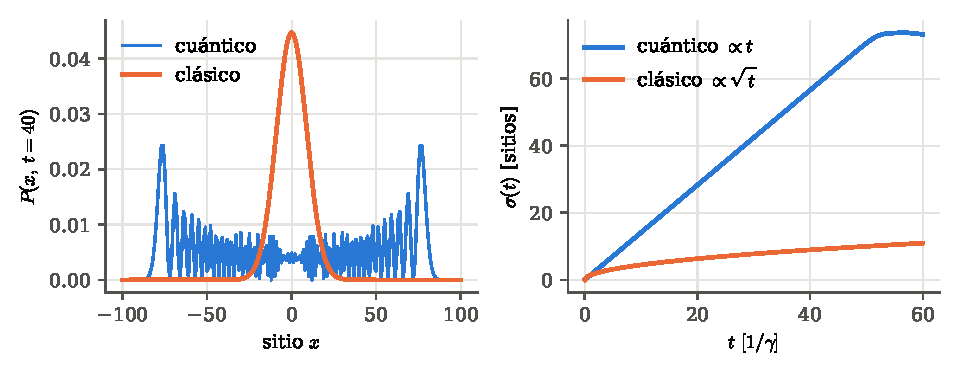
\includegraphics[width=\textwidth]{figuras/fig_cadena.pdf}
\caption{Cadena de 201 sitios con la excitación inicial en el centro. Izquierda: en $t=40$ el walk cuántico tiene dos frentes en $x\approx\pm2\gamma t$ con franjas de interferencia; el clásico es una gaussiana estrecha. Derecha: la dispersión cuántica crece linealmente hasta que el frente toca el borde ($t\approx50$).}
\label{fig:cadena}
\end{figure}

% =====================================================================
\section{El conectoma como grafo}
\label{sec:conectoma}
% =====================================================================

Los datos son las sinapsis químicas ($c_{i\to j}$) y los contactos gap ($g_{ij}$) del hermafrodita adulto de Cook \emph{et al.}~\cite{cook2019}, distribuidos por OpenWorm~\cite{openworm}. Un hamiltoniano debe ser hermítico, así que la matriz de pesos tiene que ser simétrica. El proyecto usa \emph{pesos binarios}: dos neuronas están conectadas si tienen al menos una sinapsis química (en cualquier sentido) o un contacto gap, y todas las conexiones pesan lo mismo:
\begin{equation}
W_{ij}=\begin{cases}1 & \text{si } c_{i\to j}+c_{j\to i}+g_{ij}+g_{ji}>0,\\ 0 & \text{si no,}\end{cases}
\qquad
J=\frac{W}{\lambda_{\max}(W)} .
\label{eq:J}
\end{equation}
$W$ es entonces la \emph{matriz de adyacencia} del conectoma, y el walk es el caso de libro: un CTQW sobre un grafo sin pesos.

\begin{itemize}
\item \textbf{Por qué binario.} Fue una decisión del equipo. Todas las sinapsis valen lo mismo, así que la propagación depende solo de la \emph{forma} de la red: quién está conectado con quién. La excitación salta de forma más pareja y la interferencia se reparte por más caminos. (Se puede usar en cambio $W_{ij}=\log(1+n_{ij})$ con $n_{ij}$ el número de sinapsis; el código del backend lo conserva como opción.)
\item \textbf{Normalización.} Por el teorema de Perron--Frobenius, en una matriz simétrica no negativa el mayor valor propio es también el de mayor módulo. Así $\lVert J\rVert_2=1$, la escala más rápida de la red es $\gamma$ y el tiempo queda en unidades de $1/\gamma$.
\item \textbf{Números.} $\lambda_{\max}(W)\approx32.8$; el espectro de $J$ está en $[-0.35,1]$; hay $3\,465$ pares conectados, todos con $J_{ij}=0.0305$. Un salto tarda del orden de $t\sim1/(\gamma J_{ij})\approx33/\gamma$.
\end{itemize}

\begin{honestidad}
Se pierden dos datos biológicos: la dirección de las sinapsis químicas (en el modelo la excitación puede viajar ``hacia atrás'') y cuántas sinapsis tiene cada conexión (una sinapsis y cincuenta pesan igual).
\end{honestidad}

% =====================================================================
\section{Por qué un quantum walk aparece con qubits}
\label{sec:qubits}
% =====================================================================

Hasta aquí el walk es un vector de $n$ amplitudes. El proyecto lo realiza con $n$ qubits, uno por neurona, cuyo espacio tiene dimensión $2^n$. El puente es el modelo XY.

\subsection{Hamiltoniano XY}

Con $\sigma^+=\ket1\!\bra0=\tfrac12(X-\ii Y)$ y $\sigma^-=\ket0\!\bra1=\tfrac12(X+\ii Y)$, se cumple $\sigma_i^+\sigma_j^-+\sigma_i^-\sigma_j^+=\tfrac12(X_iX_j+Y_iY_j)$: los términos cruzados se cancelan. Se define
\begin{equation}
H=\gamma\sum_{i<j}J_{ij}\,\frac{X_iX_j+Y_iY_j}{2}=\gamma\sum_{i<j}J_{ij}\bigl(\sigma_i^+\sigma_j^-+\sigma_i^-\sigma_j^+\bigr).
\label{eq:HXY}
\end{equation}

Cada término quita una excitación de una neurona y la pone en otra.

\begin{proposicion}[Conservación]\label{prop:conservacion}
El número de excitaciones $\Nop=\sum_k\sigma_k^+\sigma_k^-$ conmuta con $H$.
\end{proposicion}

\begin{proof}
$[\Nop_k,\sigma_k^\pm]=\pm\sigma_k^\pm$, de modo que $[\Nop,\sigma_i^+\sigma_j^-]=\sigma_i^+\sigma_j^--\sigma_i^+\sigma_j^-=0$.
\end{proof}

$H$ separa entonces el espacio en sectores de $k$ excitaciones, de dimensión $\binom nk$, que nunca se mezclan. El vacío $\vac=\ket{0\cdots0}$ es estacionario ($H\vac=0$), porque cada término lo aniquila.

\begin{proposicion}[Una excitación = quantum walk]\label{prop:ctqw}
Sea $\ket{e_k}=\sigma_k^+\vac$ la red con solo la neurona $k$ excitada. Entonces
\begin{equation}
H\ket{e_k}=\gamma\sum_iJ_{ik}\ket{e_i}
\qquad\Longrightarrow\qquad
\bra{e_i}\e^{-\ii Ht}\ket{e_j}=\bigl[\e^{-\ii\gamma Jt}\bigr]_{ij}.
\end{equation}
\end{proposicion}

\begin{proof}
Para $i\ne j$, $\sigma_i^+\sigma_j^-\ket{e_k}=\delta_{jk}\ket{e_i}$: solo se puede bajar la neurona que está excitada. Sumando sobre los pares y usando $J_{ik}=J_{ki}$, $H$ restringida al sector de una excitación es la matriz $\gamma J$ en la base $\{\ket{e_k}\}$. Como el sector es invariante (\cref{prop:conservacion}), su exponencial es $\e^{-\ii\gamma Jt}$.
\end{proof}

La excitación es el ``caminante'', y el walk de la \cref{sec:ctqw} es exactamente la dinámica de los qubits en este sector.

\begin{observacion}[Varios caminantes]
Con $k\ge2$ excitaciones la dinámica ya no se reduce a $J$: dos excitaciones no pueden ocupar el mismo qubit (\emph{bosones de núcleo duro}), y esa exclusión actúa como interacción. En una cadena, Jordan--Wigner lo convierte en fermiones libres; en un grafo general como el conectoma no. Los sectores crecen como $\binom{302}{2}=45\,451$ y $\binom{302}{3}=4\,545\,100$: ahí la simulación cuántica tiene sentido real.
\end{observacion}

% =====================================================================
\section{El láser y el resultado central}
\label{sec:laser}
% =====================================================================

Un pulso resonante de frecuencia de Rabi $\Omega$ y duración $\tau$ rota un sistema de dos niveles: $\RX(\theta)=\e^{-\ii\theta X/2}$, con $\theta=\Omega\tau$. Se supone que el pulso es mucho más corto que la dinámica de la red ($\tau\ll1/\gamma$).

\begin{proposicion}[Probabilidad de disparo]\label{prop:central}
Si se ilumina la neurona $j$ de la red en reposo,
\begin{equation}
\e^{-\ii Ht}\RX^{(j)}(\theta)\vac=\cos\tfrac\theta2\,\vac-\ii\sin\tfrac\theta2\sum_k\bigl[\e^{-\ii\gamma Jt}\bigr]_{kj}\ket{e_k},
\end{equation}
y la probabilidad de medir la neurona $k$ en $\ket1$ es
\begin{equation}
\boxed{\;P_k(t)=\sin^2\!\frac\theta2\;\Bigl|\bigl[\e^{-\ii\gamma Jt}\bigr]_{kj}\Bigr|^2\;}
\label{eq:central}
\end{equation}
\end{proposicion}

\begin{proof}
$\RX(\theta)\ket0=\cos\frac\theta2\ket0-\ii\sin\frac\theta2\ket1$. El vacío no evoluciona y la parte excitada hace el walk (\cref{prop:ctqw}). Como $\vac$ y los $\ket{e_k}$ son ortogonales, $P_k$ es el módulo al cuadrado del coeficiente de $\ket{e_k}$.
\end{proof}

\begin{idea}[Cómo leerlo]
La dosis de luz $\theta$ solo escala el tamaño de la respuesta: con $\theta=\pi$ el disparo es seguro, con $\theta=\pi/2$ ocurre la mitad de las veces. \emph{Qué} neuronas se encienden y \emph{cuándo} lo decide únicamente el quantum walk sobre el conectoma. Esto es exactamente lo que dibuja la animación 3D.
\end{idea}

% =====================================================================
\section{Qué hace el walk en el conectoma}
\label{sec:resultados}
% =====================================================================

\paragraph{Tiempos cortos: el orden de llegada lo fija la distancia.} En \eqref{eq:caminos}, si la neurona $k$ está a $d$ sinapsis de $j$, el primer término no nulo es $\ell=d$:
\begin{equation}
P_k(t)\approx\sin^2\!\tfrac\theta2\;\frac{(\gamma t)^{2d}}{(d!)^2}\bigl[(J^d)_{kj}\bigr]^2
\qquad(\gamma t\ll1).
\end{equation}

Las neuronas se encienden en capas según su distancia en el grafo, y dentro de cada capa ganan las que tienen más caminos cortos y más gruesos hacia la neurona iluminada.

\paragraph{Mundo pequeño: no se ve el avance balístico.} En el conectoma casi cualquier par de neuronas está a dos o tres sinapsis. La caminata clásica llega a la distribución uniforme muy rápido ($t\approx10$), así que la ventaja ``balística'' de la cadena no se nota. Lo que sí cambia, y mucho, es el tipo de distribución (\cref{fig:retorno}).

\paragraph{Cada instante es un patrón de ``speckle''.} Para tiempos largos, \eqref{eq:espectral} suma muchos términos con fases que ya no están correlacionadas, y la amplitud de cada neurona se comporta como un número complejo gaussiano. Para esa estadística (de Porter--Thomas), $\mathbb E|\psi_k|^4=2\,(\mathbb E|\psi_k|^2)^2$, y la \emph{participación efectiva}
\begin{equation}
\mathrm{PR}(t)=\frac{1}{\sum_kP_k(t)^2}\;\approx\;\frac n2\approx151 .
\end{equation}

Se observa $\mathrm{PR}\approx130$--$150$, que fluctúa sin converger. La caminata clásica, en cambio, se acerca a $n$ (distribución uniforme). En cada instante el walk cuántico tiene la mitad de las neuronas ``encendidas'' y el resto en zonas oscuras de interferencia, y ese patrón cambia todo el tiempo.

\paragraph{En promedio, el walk recuerda dónde empezó.} Si los vectores propios del conectoma se comportan como vectores reales aleatorios de varianza $1/n$, entonces $\mathbb E[V_{jm}^4]=3/n^2$ y, por \eqref{eq:promedio},
\begin{equation}
\overline{P_j}=\sum_mV_{jm}^4\approx\frac3n .
\end{equation}

Para AVM se obtiene $\overline{P_j}=3.7/n$: en promedio, la excitación pasa casi cuatro veces más tiempo en la neurona iluminada que en una neurona cualquiera, algo más que la estimación aleatoria. La caminata clásica tiende a $1/n$ y olvida. Este exceso de retorno es un efecto puramente de interferencia: los caminos que salen y vuelven por la misma ruta en sentidos opuestos llegan con la misma fase y se suman.

\begin{figure}[htbp]
\centering
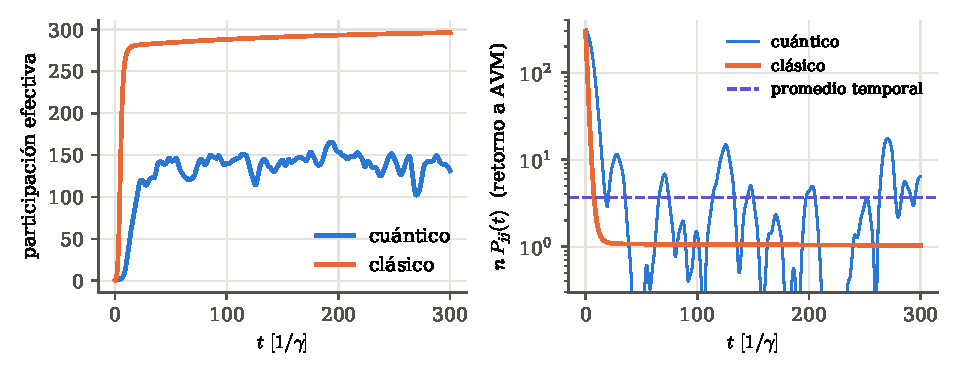
\includegraphics[width=\textwidth]{figuras/fig_retorno.pdf}
\caption{Conectoma completo, láser en AVM. Izquierda: participación efectiva; la clásica tiende a $n$ (uniforme) y la cuántica fluctúa cerca de $n/2$. Derecha: probabilidad de retorno a AVM multiplicada por $n$, en escala logarítmica. La clásica tiende a $1$ (sin memoria) y la cuántica oscila alrededor de su promedio, $3.7$.}
\label{fig:retorno}
\end{figure}

% =====================================================================
\section{Del walk al circuito (resumen)}
\label{sec:circuito}
% =====================================================================

Para ejecutar el walk en hardware se toma un microcircuito del reflejo de toque~\cite{chalfie1985}, por ejemplo \code{toque-6} = \{AVM, ALML, AVDL, AVAL, PVCL, PLML\}, con $J_S=J[S,S]$ (el mismo walk, restringido a esas neuronas y aislado del resto).

\paragraph{Un salto = una compuerta.} Para cada sinapsis $(a,b)$, $X_aX_b$ y $Y_aY_b$ conmutan, así que
\begin{equation}
\hop(\alpha)=\e^{-\ii\alpha(XX+YY)/2}=\RXX(\alpha)\,\RYY(\alpha),
\qquad
\hop(\alpha)\ket{10}=\cos\alpha\ket{10}-\ii\sin\alpha\ket{01},
\end{equation}
y deja quietos $\ket{00}$ y $\ket{11}$: es un paso del walk entre dos neuronas. En Qiskit son \code{qc.rxx(alfa, a, b)} y \code{qc.ryy(alfa, a, b)}.

\paragraph{Trotter.} Los saltos de distintas sinapsis no conmutan si comparten neurona, así que el walk completo se aproxima con $r$ pasos cortos $\delta=t/r$. Con la fórmula simétrica de Strang,
\begin{equation}
\e^{-\ii Ht}\approx\Bigl[\prod_e\hop\bigl(\tfrac{\gamma J_e\delta}{2}\bigr)\prod_{e\,\text{(al revés)}}\hop\bigl(\tfrac{\gamma J_e\delta}{2}\bigr)\Bigr]^r,
\qquad
\text{error}=O\!\left(\frac{t^3}{r^2}\right)~\cite{childs2021}.
\end{equation}

En \code{toque-6} con $r=2$ son $29$ saltos, es decir $58$ compuertas de dos qubits. Los puntos de la \cref{fig:toque6} muestran que esto ya sigue de cerca al walk exacto.

\begin{figure}[htbp]
\centering
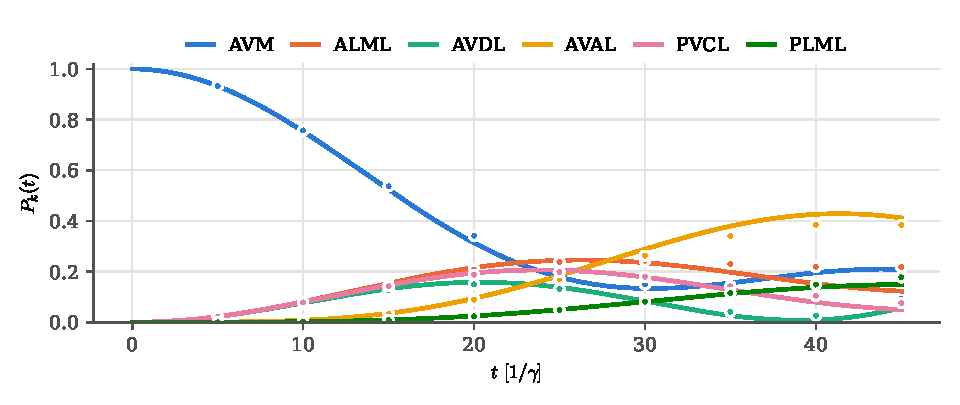
\includegraphics[width=\textwidth]{figuras/fig_toque6.pdf}
\caption{Walk exacto en \code{toque-6} desde AVM (líneas) y circuito de Trotter con $r=2$ (puntos). Se ve la excitación salir de AVM, pasar por ALML, AVDL y PVCL hacia $t\approx20$--$26$ y concentrarse en la interneurona de mando AVAL hacia $t\approx41$. El acuerdo se degrada a tiempos largos porque, con $r$ fijo, el paso $\delta=t/r$ crece.}
\label{fig:toque6}
\end{figure}

\paragraph{Givens.} Como el walk de una excitación se calcula clásicamente, también se puede \emph{preparar} su resultado con solo $n-1$ saltos, eligiendo los ángulos para repartir los módulos $|\psi_k|$ uno a uno~\cite{kivlichan2018}. Es exacto y poco profundo, pero no es simulación: necesita conocer la respuesta.

\paragraph{Conservación como control de errores.} Con un láser, ninguna medición ideal puede tener más de una neurona encendida (\cref{prop:conservacion}). Los shots que violan esa regla son errores y se descartan (post-selección por simetría~\cite{bonet2018}). En simulación con ruido tipo IonQ Forte, eso baja el error de \code{toque-6} de $0.17$ a $0.05$ (TVD). Los detalles de compilación, ruido y mitigación están en \code{teoria\_extendida.tex}.

% =====================================================================
\section{Extensiones}
% =====================================================================

\begin{itemize}
\item \textbf{Sinapsis dirigidas.} Se pueden recuperar con fases complejas $J_{ij}\e^{\ii\varphi_{ij}}$, que rompen la simetría temporal (\emph{chiral quantum walks}~\cite{zimboras2013}), o con un \emph{quantum stochastic walk}, que interpola entre el walk cuántico y el clásico~\cite{whitfield2010}.
\item \textbf{Varios caminantes.} Varios láseres a la vez llevan al régimen de bosones de núcleo duro en interacción, clásicamente costoso. El circuito de Trotter ya lo soporta.
\item \textbf{Ver la coherencia.} El estado es una superposición entre ``no pasó nada'' y ``hay una excitación viajando''. Medir en base $X$ revelaría esa coherencia, que la base $Z$ no ve.
\end{itemize}

% =====================================================================
\begin{thebibliography}{99}
\bibitem{farhi1998} E.~Farhi y S.~Gutmann, \emph{Quantum computation and decision trees}, Phys.\ Rev.\ A \textbf{58}, 915 (1998).
\bibitem{childs2009} A.~M.~Childs, \emph{Universal computation by quantum walk}, Phys.\ Rev.\ Lett.\ \textbf{102}, 180501 (2009).
\bibitem{mulken2011} O.~Mülken y A.~Blumen, \emph{Continuous-time quantum walks: models for coherent transport on complex networks}, Phys.\ Rep.\ \textbf{502}, 37 (2011).
\bibitem{cook2019} S.~J.~Cook \emph{et al.}, \emph{Whole-animal connectomes of both Caenorhabditis elegans sexes}, Nature \textbf{571}, 63 (2019).
\bibitem{white1986} J.~G.~White, E.~Southgate, J.~N.~Thomson y S.~Brenner, \emph{The structure of the nervous system of the nematode C.~elegans}, Phil.\ Trans.\ R.\ Soc.\ B \textbf{314}, 1 (1986).
\bibitem{chalfie1985} M.~Chalfie \emph{et al.}, \emph{The neural circuit for touch sensitivity in Caenorhabditis elegans}, J.\ Neurosci.\ \textbf{5}, 956 (1985).
\bibitem{nagel2005} G.~Nagel \emph{et al.}, \emph{Light activation of channelrhodopsin-2 in excitable cells of Caenorhabditis elegans triggers rapid behavioral responses}, Curr.\ Biol.\ \textbf{15}, 2279 (2005).
\bibitem{boyden2005} E.~S.~Boyden \emph{et al.}, \emph{Millisecond-timescale, genetically targeted optical control of neural activity}, Nat.\ Neurosci.\ \textbf{8}, 1263 (2005).
\bibitem{childs2021} A.~M.~Childs, Y.~Su, M.~C.~Tran, N.~Wiebe y S.~Zhu, \emph{Theory of Trotter error with commutator scaling}, Phys.\ Rev.\ X \textbf{11}, 011020 (2021).
\bibitem{kivlichan2018} I.~D.~Kivlichan \emph{et al.}, \emph{Quantum simulation of electronic structure with linear depth and connectivity}, Phys.\ Rev.\ Lett.\ \textbf{120}, 110501 (2018).
\bibitem{bonet2018} X.~Bonet-Monroig, R.~Sagastizabal, M.~Singh y T.~E.~O'Brien, \emph{Low-cost error mitigation by symmetry verification}, Phys.\ Rev.\ A \textbf{98}, 062339 (2018).
\bibitem{whitfield2010} J.~D.~Whitfield, C.~A.~Rodríguez-Rosario y A.~Aspuru-Guzik, \emph{Quantum stochastic walks}, Phys.\ Rev.\ A \textbf{81}, 022323 (2010).
\bibitem{zimboras2013} Z.~Zimborás \emph{et al.}, \emph{Quantum transport enhancement by time-reversal symmetry breaking}, Sci.\ Rep.\ \textbf{3}, 2361 (2013).
\bibitem{openworm} OpenWorm, \url{https://github.com/openworm/c302} y \url{https://github.com/openworm/CElegansNeuroML}.
\end{thebibliography}

\end{document}
